\documentclass[12pt]{article}
\usepackage{geometry}
\usepackage{xcolor}
\usepackage[utf8]{inputenc}
\usepackage{tabto}
\usepackage{graphicx}
\usepackage{pdflscape}
\usepackage{hyperref}
\graphicspath{ {./images/} }
\hypersetup{
colorlinks=false,
linktoc=all
}
\geometry{
a4paper,
left=30mm,
top=30mm,
right=30mm,
bottom=40mm
}
\newcommand{\black}{
\pagecolor{black}
\color{white}
}
\newcommand{\sentence}{} % New sentence
\newcommand{\italic}[1]{\textit{#1}}
\newcommand{\code}[1]{\texttt{#1}}
\newcommand{\fullref}[1]{\ref{#1}~\nameref{#1}}
\title{Vectorization and Compression of Animated Cartoon Videos}
\author{}
\date{}
\begin{document}

    \pagenumbering{gobble} % Remove page numbering

    \maketitle

    \begin{center}
        \vspace{5cm}
        \large
        September 2020
        \linebreak
        \linebreak
        Bassam Helal
        \linebreak
        809293
    \end{center}
    \begin{center}
        \vspace{2cm}
        
\includegraphics[scale=0.65]{SwanseaUniversityLogo.png}
    \end{center}
    \begin{center}
        \vspace{1cm}
        \normalsize
        Department of Science, Swansea University
        \linebreak
        \linebreak
        Project Dissertation submitted to Swansea University in Partial Fulfilment for the Degree of Master of Science
    \end{center}

    \pagebreak

    \begin{center}
        \section*{Abstract}
    \end{center}
    Preserving media made by those who preceded us is an important duty that we must do our best to
    accomplish, as during that moment we are the keepers of and choosers of history.
    \sentence
    Cartoons an excellent example of this, a form of media created and pioneered by our ancestors that have shaped
    our lives and will shape the lives of our children and those who follow us.
    \sentence
    Cartoons are currently stored using the most prevalent format, raster graphics, a format that is susceptible to
    aging due to its issues with scaling on newer higher resolution displays.
    \sentence
    As time goes on and these displays continue to increase in resolution, the risk of older media becoming unusable,
    obsolete or simply unwatchable increases more and more, risking future generations to be unaware or uninterested
    in otherwise masterpieces of art and culture.
    \sentence
    One way of tackling this dire problem, is by converting the media into an infinitely scalable format that they
    are well suited to, vector graphics which will in addition allow them to take up less disk space.
    \sentence
    There have been existing attempts at performing this task and many continue to be researched and developed such
    as those made by the ever popular machine learning computational model.
    \sentence
    But with machine learning comes a dependence on a training dataset leading to a model that is neither sustainable
    nor general purpose and will only succeed on the data it is trained against.
    \sentence
    This project attempts to tackle this problem by experimenting with different methods and techniques to convert
    the data into vector formats and while doing so reduce its size as well.
    \sentence
    While results are very promising, there is still more to explore and discover, the problem we are facing is more
    challenging and complex than it seems.
    \sentence
    But it is a necessary struggle as it may make be the small push needed to help create a method of preserving
    these cultural and historic treasures that we grew up with and loved and hopefully live to watch our descendents
    enjoy them as much as we did, no matter the technology difference.

    \pagebreak

    \begin{center}
        \section*{Declarations}
    \end{center}
    \subsection*{Declaration}
    This work has not previously been accepted in substance for any degree and is
    not being concurrently submitted in candidature for any degree.

    \subsection*{Statement 1}
    This dissertation is the result of my own independent work/investigation, except
    where otherwise stated.
    Other sources are acknowledged by giving explicit references.
    A bibliography is appended.

    \subsection*{Statement 2}
    I hereby give consent for my dissertation, if accepted, to be available for
    photocopying and for inter-library loan, and for the title and summary to be
    made available to outside organisations.

    \bigskip
    \begin{figure}[h!]
        \centering
        
\includegraphics[width=0.4\textwidth]{Signature.png}
        \linebreak
        \today\label{fig:signature}
    \end{figure}

    \newpage

    % TODO 12-Sep-20 Abstract

    \pagebreak

    \renewcommand*\contentsname{
    \begin{center}
        Table of Contents
    \end{center}}

    \tableofcontents

    \pagebreak

    \pagenumbering{arabic} % Begin page numbering from here


    \section{Introduction}\label{sec:introduction}

    \tab
    Moving pictures have existed for at least 100 years and have been a prevalent and important part of our lives for
    generations from films to broadcast television to online video.
    \sentence
    As display technology improves, so does the need for higher fidelity media to make use of the new displays,
    whether it be higher color quality, higher resolutions, or higher framerates, the evolution of technology never
    stops.
    \sentence
    However, as this technology improves, media made for older technology becomes more and more dated showing its age
    and slowly becoming closer to obsolescence and near unusable.
    \sentence
    And while digitization allows these media to live a longer life in its original form, it does not allow the media
    to age well as display technologies inevitably improve.
    \sentence
    Cartoons are a form of media that show much less signs of these symptoms, remaining relevant and watchable well
    past other media from their time, \italic{Tom and Jerry} is the perfect example of this.
    \sentence
    But with the ever increasing desire for higher fidelity moving picture, even once thought timeless media has
    begun to show its age with some modern displays.
    \sentence
    Just as preserving this media in its original form is important, so too should aiming to maintain it to live for
    future generations as if it were made for them and not from an era long gone.

    \bigskip
    This project aims to tackle this issue, namely, try to transform cartoons into a form that can live and scale to
    the displays of the future not just the present.
    \sentence
    This is achieved by using one of the most powerful graphics format that, if used correctly, can create graphics that
    scale infinitely \italic{and} have a small file size, vector graphics.
    \sentence
    Cartoons are not stored in this format and are instead stored using the ubiquitous raster graphics formats, thus
    a process must be developed that can transform the cartoons from raster graphics to vector graphics.
    \sentence
    This process must be both as accurate as possible to the original \italic{and} have reasonable storage costs,
    ideally smaller than any alternative.
    \sentence
    This project aims to develop just that, to transform cartoons from raster graphics to vector graphics (a process
    known as vectorization) and do so aiming for the highest accuracy while also achieving a smaller file size as a
    result.

    \bigskip
    There already exists existing research and applications for both vectorization and compression with a great deal
    of advancement using machine learning techniques in addition to the existing techniques.
    \sentence
    Vectorization is used across many different fields and disciplines to convert data captured in raster graphics
    into vector graphics in order to be better used for analysis and processing.
    \sentence
    Modern research has begun exploring machine learning based methods to convert raster based images into vector
    graphics with very high accuracy and filtering.
    \sentence
    Compression too has been heavily researched and developed since the early 90s and new research has emerged also
    using machine learning to heavily increase space savings while also \italic{increasing} picture quality beating
    traditional methods by a big margin.
    \sentence
    These developments and research will only continue to grow and improve meaning that this problem is becoming
    closer and closer to being solved as more people tackle it with different approaches.

    \bigskip
    However, the existing research and applications do not tackle the vectorization problem in an ideal fashion and
    machine learning approaches bring with them the issues of the machine learning computational model.
    \sentence
    Existing vectorization methods often make a compromise between file size and accuracy, usually in order to be as
    general purpose as possible.
    \sentence
    Machine learning approaches will always bring with them the failures of machine learning which is too dependent
    and affected by the learning dataset and is seen as a black box of unknown computation.
    \sentence
    This project attempts to remedy this by developing a vectorization process specifically aimed at cartoons with no
    machine learning involved in order to have a fully transparent, portable and sustainable process.

    \bigskip
    After months of research and development results have shown that the process is much more difficult than
    anticipated but still theoretically feasible without the need for any machine learning.
    \sentence
    These positive results are still far from perfect as there have been many unexpected challenges and issues faced
    that reduce the impressiveness of the results and prove to show that the project is much more challenging than it
    may seem.
    \sentence
    However despite that, the results show that it is technically possible to achieve some fairly impressive results
    and perhaps given more time to properly develop and optimize the process, even greater results would follow.

    \bigskip
    This document will cover the story of several months of research and development from the necessary background
    knowledge to the results and reflection.
    \sentence
    Section~\fullref{sec:background} covers the necessary background knowledge needed followed by
    section~\fullref{sec:related-work} which goes over some of the existing research and applications.
    \sentence
    Section~\fullref{sec:implementation} goes in detail surrounding the technical implementation details and methods.
    \sentence
    Section~\fullref{sec:software-engineering} covers the important software engineering aspects of the project's
    management, important for this project as it is part of an \italic{Advanced Software Technology} degree.
    \sentence
    Sections~\fullref{sec:evaluation} and~\fullref{sec:results} go over defining evaluation methods and describing
    the results of the project respectively.
    \sentence
    Sections~\fullref{sec:challenges},~\fullref{sec:reflection} and~\fullref{sec:future-work} reflect back on the
    challenges and experiences of the project and detail the possible endeavours the project can overcome in the future.
    \sentence
    Finally, section~\fullref{sec:conclusion} wraps up the document and concludes with final thoughts moving forward.

    \pagebreak


    \section{Background}\label{sec:background}

    \tab
    This document makes no assumption of the reader's knowledge in computer graphics and its related fields,
    thus, this section will introduce the reader to some of the required knowledge needed for understanding this
    project.
    \sentence
    Firstly, we will introduce raster graphics, the current de facto standard for graphics data representation.
    \sentence
    We will then introduce its counterpart vector graphics, a different way to store graphics data that addresses
    some of the issues with raster graphics.
    \sentence
    We will then give a brief primer on image compression and some common methods of reducing the overall size
    of an image.
    \sentence
    Finally, we will explain how image graphics tie into video graphics and describe some of the few differences
    between the two.

    \subsection{Raster Graphics}\label{subsec:raster-graphics}

    \tab
    Raster graphics is the current most popular way of representing and storing graphics data.
    \sentence
    This representation format stores the image data as a grid of pixels, a pixel (picture element) being the
    smallest element of the image containing the color information of the image at a particular point in the grid\cite{foley1994introduction}.
    \sentence
    Colors can be represented in many different formats but the most common is the three channel RGB (Red, Green, Blue)
    with RGBA (Red, Green, Blue, Alpha) gaining popularity.
    \sentence
    Each channel has a bit depth which details the number of possible colors that the channel can contain with 8 bits
    per channel being the current most common but higher values exist as well such as 10 and 12 bits per channel\cite{foley1994introduction}.
    \sentence
    So a pixel in RGB format is really just a 3-tuple (triple) of numbers for each color channel in that pixel.
    \sentence
    An image's resolution is the number of total pixels it contains, which is the image's width multiplied by its
    height, higher resolution images have more detail but are also more expensive to store as there is more data.
    \sentence
    While these concepts are seen as the current norm in computer graphics, they are more specific to raster graphics
    in particular.
    \sentence

    \bigskip
    Raster graphics are the most popular form of image and generally graphics representation as they are easy to
    understand and display.
    \sentence
    The main disadvantages of raster graphics concern image resolution and detail, namely that images will show
    pixelation artifacts when they are displayed at a higher resolution than their own where the image will start
    showing the raw pixels.
    \sentence
    To match the evolving increase in display resolutions, newer media uses higher resolutions in order to show
    optimally on these displays but at a cost.
    \sentence
    The first cost being that the new higher resolution images require more disk space to store as they are larger in
    size, but the less obvious cost is that it leaves the older lower resolution content behind.
    \sentence
    Any content made in low resolutions will forever live with that resolution and continue to scale more poorly as
    displays have higher resolutions.
    \sentence
    Therefore, while raster graphics are the current de facto standard for graphics representation, they are not
    without their major disadvantages, namely concerning the need for increased resolutions, meaning more disk space
    needed and old content becoming more and more outdated.
    \bigskip
    \begin{figure}
        
\includegraphics[width=0.45\textwidth]{Raster1.png}
        
\includegraphics[width=0.55\textwidth]{Raster2.png}
        \caption[Pixelation]{Pixelation occurs when displaying a raster image at a higher resolution than its own}
        \label{fig:pixelation}
    \end{figure}

    \subsection{Vector Graphics}\label{subsec:vector-graphics}

    \tab
    Another graphics representation format is vector graphics, which addresses some of the issues of raster graphics
    and is growing in popularity within some domains.
    \sentence
    Vector graphics uses a more declarative style of data storage, where instead of storing the data to be shown
    (such as pixels containing color information), vector graphics is based on instructions to a renderer
    about how to draw the image\cite{ferraiolo2000scalable}.
    \sentence
    These instructions are based on a set of standard geometric elements that are used in that vector graphics format
    or protocol.
    \sentence
    The most common and well known vector graphics format today is SVG, Scalable Vector Graphics, which is developed
    by the W3C since 1999, this is the format we will be using throughout this document when referencing vector
    graphics\cite{ferraiolo2000scalable}.
    \sentence
    An SVG file is nothing more than an XML-like text file with XML elements part of the SVG standard that describe
    to the renderer how to draw the image.
    \sentence
    The SVG specification defines many elements that can be used in an SVG file but the most important one in our
    case is the SVG \code{path} element\cite{noauthor_paths_nodate}.
    \sentence
    The \code{path} element can be used to draw a complex line by providing it with commands on where and how to
    draw, it is perhaps the single most powerful element within the SVG specification and is the only element that we
    will use in this project\cite{noauthor_paths_nodate}.
    \sentence

    \bigskip
    The greatest advantages of vector graphics that they address the main issues of raster graphics mentioned in
    section~\fullref{subsec:raster-graphics}, that is to say that vector graphics are resolution independent
    and are (theoretically) infinitely scalable no matter the display\cite{ferraiolo2000scalable}.
    \sentence
    The scalability of vector graphics actually solves both issues at once because there is no longer a need for
    higher resolution media thus saving on disk space \italic{and} keeping old media still usable because of infinite
    scalability.
    \sentence
    But such advantages don't come with some issues, and there's a reason vector graphics are not the current norm.
    \sentence
    Simply put, vector graphics are only good at displaying certain kinds of images and media because of the way they
    represent data, making it very difficult to accurately and efficiently store other kinds of images such as images
    of natural scenery or faces\cite{noauthor_raster_nodate}.
    \sentence
    This is because those kinds of images tend to have a large degree of color fluctuations and especially
    non-linear, complex color fluctuations.
    \sentence
    This is a particular weakness of vector graphics and one that has limited its adoption and growth because
    compared to raster graphics in this regard, vector graphics are significantly inferior.
    \sentence
    As a result, vector graphics are seen as mostly domain and use-case specific and not general purpose, they are
    excellent for logos and icons specifically because of their scalable nature but are inferior when used for
    photographs because of the complex color fluctuations of those images.

    \begin{figure}[h]
        \centering
        
\includegraphics[width=0.3\textwidth]{ChromeRaster.png}
        
\includegraphics[width=0.3\textwidth]{ChromeVector.png}
        \caption[Chrome]{Vector graphics are very practical for logos, the vector graphics image on the right scales
        significantly better than its raster counterpart on the left and has a smaller size too (4kb vector, 50kb
        raster)}
        \label{fig:chrome}
    \end{figure}
    \begin{figure}[h]
        \centering
        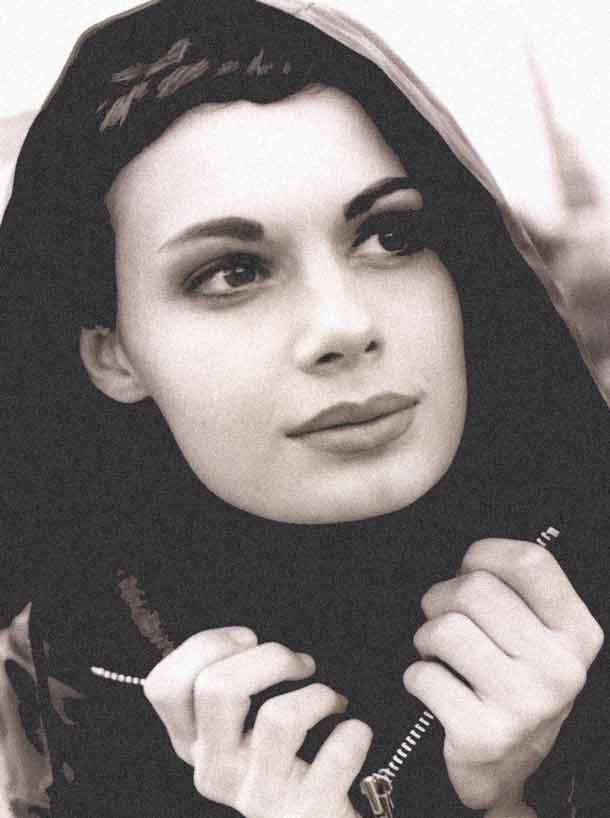
\includegraphics[width=0.3\textwidth]{WomanRaster.jpg}
        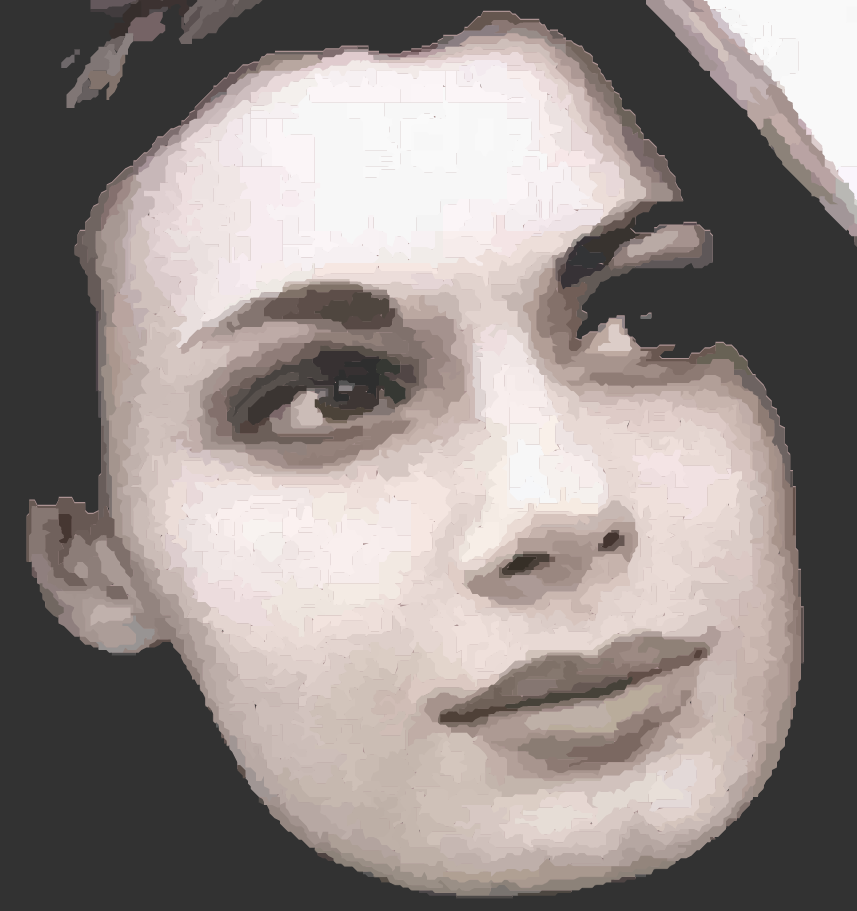
\includegraphics[width=0.3\textwidth]{WomanVector.png}
        \caption[Woman]{Vector graphics suffer with high tone fluctuation images, the vector image on the right is
        worse and larger in size than its raster counterpart on the left (25kb raster, 1MB vector)}
        \label{fig:woman}
    \end{figure}

    \subsection{Image Compression}\label{subsec:image-compression}

    \tab
    One of the most important subjects within computer graphics is image compression, that is reducing the file size
    of an image.
    \sentence
    Image compression concepts are fundamentally identical to those of classical file compression but to ensure the
    reader is up to date, we go over some of these briefly in addition to one novel concept somewhat specific to
    image compression.
    \sentence
    Compression really comes in two major forms, both relating to the data loss that happens after the compression
    process is completed, lossy compression and lossless compression.
    \sentence
    Lossy compression removes data during the process of compression to make the most of the reductions, usually
    this is redundant or unnecessary data depending on the context or domain.
    \sentence
    For example audio compression algorithms will typically remove frequencies beyond the human hearing range,
    removing unnecessary data.
    \sentence
    In the graphics world this is what is known as \italic{visually lossless compression} which means visually, to
    the human eye, no data was lost, although technically the algorithm is lossy and data was actually lost\cite{rabbani_digital_1991}.
    \sentence
    Because of its lossy nature, lossy compression is a one way process that will have irreversible data loss such
    that attempting to compress again using lossless compression will not regain the lost data.
    \sentence
    Lossless compression on the other hand, aims to reduce file sizes without any loss of data, a more difficult task
    to achieve with often worse compression ratios than lossy compression algorithms.
    \sentence
    The compression ratio of a compression algorithm is the ratio of the uncompressed size to the compressed size but
    space savings is also popular as it is more indicative of the effects of compression.
    \sentence

    \bigskip
    Image compression is used by all popular image formats to have more reasonable sizes.
    \sentence
    Lossy formats include JPEG and GIF which will show compression artifacts if encoded many times successively
    showing the data loss upon each compression pass, these formats are excellent for portability and transfer and
    indeed have been very popular on the web where bandwidth and data caps are noteworthy\cite{rabbani_digital_1991}.
    \sentence
    Lossless formats include BMP and PNG which will always retain their data even after successive compresses, these
    formats however offer less compression compared to the lossy formats but are useful for those who need the
    highest quality with the guarantee of no data loss\cite{rabbani_digital_1991}.
    \sentence
    These concepts are essentially identical to those found in classic file compression with the exception of
    \italic{visually lossless compression} being a lossy compression method that aims to be "lossless to the human
    eye" which is preferred if lossy compression is the compression method of choice.

    \subsection{Vectorization}\label{subsec:vectorization}

    \tab
    Converting graphics from raster to vector allows for one to make use of the benefits of vector graphics and is a
    used by people across multiple domains, this process is known as vectorization or raster-to-vector conversion.
    \sentence
    This process is often used by specialists when viewing image data captured in raster to be viewed by a vector
    graphics program that can then perform additional processing such as classification, labelling etc.
    \sentence
    This process is, by its nature, lossy, meaning the original data will be lost during the process because the
    process is transformative and even though a lossless process is theoretically possible, it would not be practical
    or efficient as it would not introduce any of the benefits of vector graphics and would instead just be
    converting pixels into pixels in vector graphics\cite{vectortoraster}.
    \sentence
    Therefore, the process aims to be \italic{Visually Lossless} aiming for highest accuracy while also trying to
    effectively and efficiently transform the data into suitable optimal vector graphics data\cite{vectortoraster}.
    \sentence
    This will often mean trying to undo rasterization effects or artifacts in order to achieve a better output that
    makes sense in a vector format such as for example, interpolating pixels in order to create smooth lines
    or doing some kind of color reduction, both of which change the original data in order for it to make more sense
    in the vector output.

    \bigskip
    \sentence
    In that vain, it is also important to note that the vectorization process will also be dependent on the input
    data provided with images that do not have vectorizable qualities resulting in poor vector results, either in
    terms of accuracy or file size or both.
    \sentence
    These kind of images are most often photographs or other kinds of images with a high degree of color fluctuations
    as mentioned in section~\fullref{subsec:vector-graphics}.
    \sentence
    Whereas images with discrete color regions such as logos, icons and other "man-made graphics" often contain less
    of these qualities and will more likely do well in the vectorization process because the vectorization process
    does not work well on color fluctuations.
    \sentence
    In such cases raster graphics is always a better format as it will much more effectively store such data with
    high clarity and lower file sizes, as such, it is important for one to know where each format is more suitable as
    they each have their advantages and disadvantages.
    \sentence
    Knowing that however, when one does deduce that vector graphics is the more suitable format for their graphics,
    vectorization will allow those people to convert their graphics from raster to vector in a manner that is as
    effective as possible in order to obtain visually lossless transformation that will still be optimal as a vector
    graphics output.

    \bigskip
    \begin{figure}[h]
        \centering
        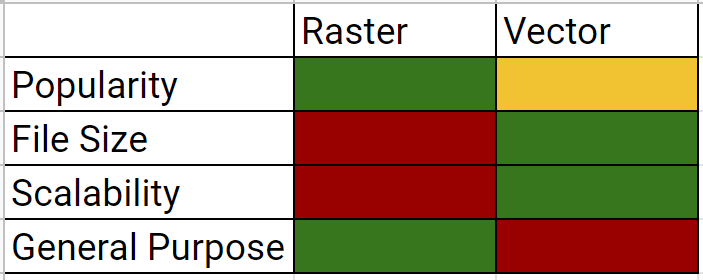
\includegraphics[scale=0.6]{Comparison.png}
        \caption[Comparison]{A chart comparing some properties between raster and vector graphics, while raster
        graphics is most popular, vector graphics have grown in popularity within some domains}
        \label{fig:comparison}
    \end{figure}

    \subsection{Video Graphics}\label{subsec:video-graphics}

    \tab
    There is a reason we have only described image graphics specifically and not mention videos and
    that is because for the most part, the two are very interchangeable as videos are essentially a series of
    sequential images.
    \sentence
    The most obvious difference being twofold, videos are temporal, meaning they are concerned with time, and videos
    contain audio data in addition to the visual graphical data.
    \sentence
    For this project we will completely ignore the audio aspects of videos and remain only concerned with the visual
    properties of videos, ie the "moving pictures" part.
    \sentence
    While it is true that videos are essentially a series of images, raster images specifically, different formats
    and codecs will store the video data differently in order to optimize for quality, compression or both.
    \sentence
    One such codec, the popular MPEG and its derivatives, explicitly make use of video's temporal nature in order to
    find and eliminate redundant data to increase compression rate while minimizing quality loss\cite{richardson2004h}.
    \sentence
    This essentially aims to group similar frames into a frameset and instead of storing all the frames, store only
    the difference between the frames which is especially effective when the frames are very similar to one another.
    \sentence
    These codecs also perform a wide variety of other smart operations to maximize compression rate while minimizing
    quality loss when doing so because of the main daunting issue with video, video is naturally very storage
    expensive\cite{richardson2004h}.
    \sentence
    This issue continues to compound as display resolutions continue to increase and raster media keeps catching up
    to it showing the same issues mentioned with raster graphics in section~\fullref{subsec:raster-graphics}.
    \sentence
    In addition to this, video media is ever-growing in popularity and ubiquity, especially on the web, making the
    demand for high fidelity, low bandwidth consuming video higher than ever.
    \sentence
    Despite these smart compression focused codecs however, video graphics concepts are largely identical to those of
    image graphics with video being simply a series of sequential images that can be encoded in many different ways
    for optimal compression and quality.

    \subsection{Libraries}\label{subsec:libraries}

    \tab
    This project uses a variety of popular tools and libraries to achieve its aims and objectives both efficiently
    and quickly, this section will briefly go over the most important tools used.
    \sentence
    This project uses Node.js as its runtime platform, Node.js is a cross-platform runtime environment that executes
    JavaScript code on a machine instead of the usual JavaScript runtime, the browser\cite{node.js_about_nodate}.
    \sentence
    The choice for Node.js was made paradoxically because of both a familiarity with the runtime and the JavaScript
    ecosystem as well as a strong desire to further enhance our knowledge and experience in both the platform and
    ecosystem.
    \sentence
    Node.js uses JavaScript as its runtime language\cite{node.js_about_nodate}, while JavaScript is a powerful and
    excellent language for rapid-prototyping, it is also a very error-prone language as it has no typing checks in place.
    \sentence
    TypeScript is a programming language that is a strict superset of JavaScript that adds typing features onto
    JavaScript and transpiles to performant, cross-platform compatible JavaScript by means of a TypeScript compiler\cite{noauthor_typed_nodate}.
    \sentence
    TypeScript was chosen as the programming language of choice for the project for its many benefits not limited to
    its added type safety.
    \sentence

    \bigskip
    \sentence
    Node.js also allows us to access the ever-growing JavaScript ecosystem which includes libraries and
    frameworks for both the front-end and back-end side of development, of which this project makes use of some
    notable tools such as Electron, GPU.js and OpenCV among others.
    \sentence
    Electron allows developers to write desktop applications using web technologies, it is essentially a Chromium
    browser with two processes, a front-end process called the "renderer" which is similar to a Chromium web page
    that displays HTML, and a back-end process called the main process which is a Node.js process\cite{noauthor_electron_nodate}.
    \sentence
    Electron combines Node.js and Chromium to allow a developer to write a native desktop application using the same
    technologies used on the web, this has its own advantages and disadvantages but in our case, it means we can
    quickly develop a GUI desktop application that can access our Node.js code without resorting to web servers and
    other more complicated means\cite{noauthor_electron_nodate}.
    \sentence
    GPU.js is a JavaScript library that allows developers to run code on the host machine's GPU making use of the
    GPGPU (General-Purpose computing on Graphics Processing Units) paradigm to allow for very large performance
    improvements and speedups for computationally expensive mathematical operations\cite{noauthor_gpu.js_nodate}.
    \sentence
    In summary, the project uses the Node.js runtime for its large ecosystem, the TypeScript programming language for
    its added type safety benefits, Electron to easily display a GUI and GPU.js to run code on the GPU for additional
    performance when needed.
    \pagebreak


    \section{Related Work}\label{sec:related-work}

    \tab
    Vectorization has existed for some time now and there is much ongoing and existing research aimed at finding new
    ways of improving the process for higher accuracy and lower file sizes.
    \sentence
    There also exist real world applications in industry using vectorization methods ranging across domains such as
    art to medicine.
    \sentence
    This is also the case for image and video compression as well since resolutions are ever increasing and with them
    come increased file sizes that are needed to be controlled in order to keep storage space costs low.
    \sentence
    This section will firstly detail some of the existing and current research done within the realm of image
    vectorization and compression in section~\fullref{subsec:current-research}.
    \sentence
    Next, we will go over some of the existing applications of vectorization as well existing compression algorithms
    in section~\fullref{subsec:current-applications}.
    \sentence
    Finally, we mention some of the limitations and flaws with the existing technologies within the realm of
    vectorization in section~\fullref{subsec:existing-limitations}.

    \subsection{Current Research}\label{subsec:current-research}

    \tab
    The existing and current research within image vectorization continues to improve and grow with time,
    particularly in the current age of machine learning where results can truly become revolutionary.
    \sentence
    Some of the most interesting research comes in the form of converting sketches into digital art through the means
    of vectorization by making use of machine learning using adversarial neural networks~\cite{masteringsketch}.
    \sentence
    This algorithm can especially distinguish between noise, light strokes, heavy strokes and fill in the gaps that
    are found from pencil drawings.
    \sentence
    While the intended purpose is for sketch artists, the possible future use cases are quite remarkable including
    general purpose vectorization.

    \bigskip
    In addition to vectorization, image and video compression research has been thriving and growing and it
    too has also been bolstered in the current age of machine learning.
    \sentence
    In recent years there have been novel developments in image compression using machine learning that can produce
    files more than 2 times smaller than those produced by JPEG compression~\cite{rippel2017}.
    \sentence
    This is made possible through the help of machine learning techniques that are becoming more and mainstream
    within the research community to try to improve compression rate over traditional methods.
    \sentence
    By using machine learning, research has proven that we can improve compression rates by a significant amount and
    have better quality images than traditional algorithms showing that machine learning produces very high quality
    results in the compression realm.

    \subsection{Current Applications}\label{subsec:current-applications}

    \tab
    In addition to the existing research there also exist many real world applications in industry that
    use vectorization in parts of their application or service.
    \sentence
    Potrace is one the oldest and most well known applications that can convert raster images to monochrome vector
    graphics formats with high performance\cite{noauthor_peter_nodate}.
    \sentence
    It is used across many different applications and service most notably Inkscape, one of the most popular vector
    image editors to date.
    \sentence
    Vectorization is also used generally across multiple fields and disciplines to convert raster image data into a
    domain specific format that can more easily be analyzed and processed by specialists or computers alike.
    \sentence
    The means vectorization is widely used for many different purposes and these tools are some of the ways this can
    be done in the real world.

    \bigskip
    In addition to vectorization there also exist a vast multitude of image and video compression algorithms and
    codecs that aim to achieve the highest space savings while maintaining the highest level of quality at the same
    time.
    \sentence
    Perhaps the most important and most influential of these being the JPEG format which continues to be the most
    widely used image compression standard since its inception in 1992\cite{pennebaker1992jpeg}.
    \sentence
    JPEG aims for visually lossless compression by using the Discrete Cosine Transform which itself is also used for
    compression across other popular codecs such as those developed by the MPEG group as well as the H.26x codecs\cite{richardson2004h}.
    \sentence
    There continue to be more developments towards formats that can perform even better compression with less quality
    loss \italic{and} with fast encode times (for videos) such as the very recently developed H.266 video codec.
    \sentence
    These algorithms, formats and codecs continue to evolve and improve showing that image and video compression also
    continues to remain a relevant and important problem to tackle as higher resolution displays continue to emerge
    and become ubiquitous.

    \subsection{Existing Limitations}\label{subsec:existing-limitations}

    \tab
    While the aforementioned current research and applications are very impressive and revolutionary, they are not
    without their limitations or issues, especially some of the latest research using machine learning as they will
    inherit the limitations and issues that come with that computational model.
    \sentence
    With the age of machine learning there has been a growing desire to solve every problem using machine learning
    and leave behind the days of old where solving a problem by hand was the only way.
    \sentence
    However, as more applications and services use machine learning to solve their problems, sometimes already solved
    problems, the inherent flaws that come with machine learning make themselves more and more apparent.
    \sentence
    Machine learning is still extremely dependent on the materials that were used to train it and this is in fact a
    requirement for a machine learning algorithm, it needs a lot of existing data to be trained, something that may
    not be readily available.
    \sentence
    Machine learning is also trained well based on the input data provided but will perform poorly if given data it
    has not seen before, even if that data is still relevant.
    \sentence
    In this case the solution is to get more training data and retrain the model until it has learned but this
    solution is not sustainable and not cheap as machine learning training is very computationally expensive.
    \sentence
    Not always is there readily available datasets to be used for training and it is not feasible to always be
    retraining the model when some new input data is used that it has never seen.
    \sentence
    This is all without mentioning that with machine learning there is no idea at all what is happening and how the
    machine is processing the data, there is a black box between the input and the output, something that is
    absolutely not maintainable or sustainable in the long term.
    \sentence
    Therefore, not all problems can be solved using machine learning and it is important to recognize the inherent
    flaws and limitations of machine learning as well as the dangers of trusting machine learning to solve every
    problem as this leads to no understanding of any of the processing.

    \bigskip
    Non machine learning based algorithms are still not without fault however, as there exist limitations
    inherent to the vectorization process that have not yet been solved.
    \sentence
    Potrace can only output monochrome images, completely ignoring colors entirely and even then will still not fully
    accurately trace the edges correctly because internally it using edge detection in order to draw the edges.
    \sentence
    Other algorithms such as ImageTracer.js will either achieve high accuracy at the cost of file size, or small file
    sizes at the cost of accuracy and with some required parameters such as desired number of colors.
    \sentence
    While these algorithms do perform the vectorization process as advertised, they still do not overcome some of the
    inherent issues with the process and thus still are limited in their usefulness for vectorizing animated cartoons
    in a way that is both accurate and size optimal.

    \pagebreak


    \section{Implementation}\label{sec:implementation}

    \tab
    The following section will go into high level detail describing the implementation details of the project.
    \sentence
    While this section may seem rather long, it is in fact made dense to ensure conciseness while keeping all the
    necessary details explained.
    \sentence
    This is because the project explores many different ideas and implementations to try to achieve its goals as will
    be evident by the multiple vectorization methods used.
    \sentence
    Firstly, we introduce the high level process pipeline of the project from input to output.
    \sentence
    Then, we explore in depth some of the many methods of vectorization used in the project.
    \sentence
    Finally, we describe the limitations and drawbacks that were found during the implementation.

    \subsection{Pipeline}\label{subsec:pipeline}

    \begin{figure}[h]
        \centering
        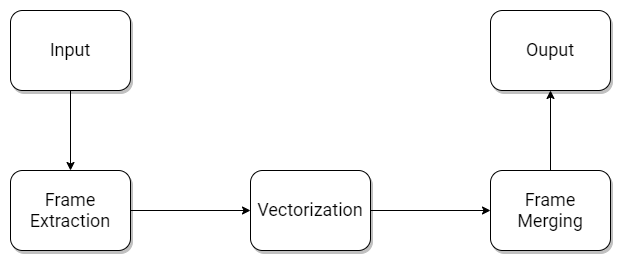
\includegraphics[width=\textwidth]{Pipeline.png}
        \caption[Pipeline]{Process pipeline}
        \label{fig:pipeline}
    \end{figure}

    \bigskip

    The above image shows the high level process pipeline of the project from input to output with each phase of the
    pipeline further detailed in its own section below.
    \sentence
    Firstly, we explain the expected input video and its ideal characteristics that will result in a higher accuracy
    output.
    \sentence
    Then, we establish the expected and desired output and detail its expected and ideal characteristics before
    further discussing any of the processing.
    \sentence
    Then, the first phase of the processing begins, the frame extraction, where the frames of the video are
    extracted to be used further down the pipeline.
    \sentence
    Next, the main phase of the processing, the vectorization of a single frame, we describe and detail the multiple methods
    and approaches that were used in order to gain the highest level of accuracy and compression rate on each frame.
    \sentence
    Finally, the final stage of the processing, frame merging combines the vectorized frames back into a playable
    video form with additional computation executed to add favorable traits such as further reduced file sizes.

    \subsubsection{Input}\label{subsubsec:input}

    \tab
    Firstly, it is important to understand the input that the process will be expecting and detail what makes an ideal
    input file that will produce the best results.
    \sentence
    The minimum requirement is that the input file be any video, but more specifically, this project
    aims to work on animated cartoons, so while any video will technically work, for the purpose of this project, a
    video of an animated cartoon is expected.
    \sentence
    However, not all animated cartoons are equal, in fact there is a great deal of variation between cartoons in
    terms of art style, animation method, and many other artistic effects that can heavily influence the output of
    the process.
    \sentence
    Thus, we must define the "ideal" input file, or more precisely, the input file that will produce the best results
    because the process was designed with those files in mind for reasons to do with the limitations of vectorization.
    \sentence
    The ideal input video is one that is most friendly towards vectorization, meaning it has the most vectorizable
    qualities and characteristics with as few incompatibilities as possible, these were mentioned in depth
    in section~\fullref{subsec:existing-limitations} but will be briefly repeated within this new context.

    \bigskip
    Since vectorization is heavily dependent on the color variation of the original raster image, an ideal input
    image would be one with discrete color regions made up of a single color, with no noise, gradients, shadows,
    lighting or any other effects, essentially an image made of a set of color blocks that are very discrete from one
    another.
    \sentence
    In addition to this, it is important to note that we are dealing with moving pictures and it is also ideal to
    have as little noise as possible \italic{between} frames, this can be an artifact of compression or
    rasterization but can also be seen as an artistic style choice as shown in Cartoon Network's
    \italic{Ed, Edd n Eddy}.
    \sentence
    Obviously very few real world media satisfies these conditions, but a surprising number of cartoon videos can come
    very close to this description, with very few complications such as shadows and light gradients that are usually
    in the background or are less important elements of the image.
    \sentence
    An example of a real world cartoon that has these ideal qualities is Nickelodeon's \italic{The Fairly OddParents}
    which uses discrete color regions, very few (if any) gradients and no complex shadows or lighting.
    \sentence
    On the other extreme end cartoons with heavy use of photographs or heavy noise are the least ideal as well as
    any 3D cartoons, ie those that make use of 3D effects such as shadows, lighting and many complex gradients.
    \sentence
    Examples include Hanna Barbera cartoons prominent from the 1960s to the 1980s such as \italic{Top Cat}
    and\italic{The Flinstones} and modern 3D animations such as Pixar Animation Studios'
    \italic{Toy Story} and \italic{The Incredibles}.
    \sentence
    In summary, the minimum required input is simply any video but the expectation is that it will be an
    animated cartoon video and the ideal input being an animated cartoon video that has highly vectorizable qualities.

    \bigskip
    \begin{figure}[h]
        \centering
        
\includegraphics[width=0.95\textwidth]{FairlyOddParents.jpg}
        \caption[Fairly Odd Parents]{\italic{The Fairly OddParents} is stylized with discrete color regions making it
        ideal for vectorization}
        \label{fig:fairlyoddparents}
    \end{figure}
    \bigskip

    \subsubsection{Output}\label{subsubsec:output}

    \tab
    Before discussing any of the processing, it is important to first understand the expected output that the process
    will generate and detail the expected and ideal characteristics of the output.
    \sentence
    In essence, the output is a playable video that uses vector graphics to store the same data as the input file but
    with the added benefits of vector graphics, namely improved scalability and reduced size.
    \sentence
    Ideally, the output will be visually indistinguishable from the original but with a smaller size essentially
    achieving so called~\italic{Visually Lossless Compression}.
    \sentence
    However, since the video is using vector graphics, it will be much more scalable in comparison and essentially
    void of the pixelation problem that plagues traditional raster graphics.
    \sentence
    The size difference should especially be evident when taking the upscaling ability into account since the new
    video can be effective at any resolution display whilst the original will show pixelation once it is displayed on
    high enough resolution displays.
    \sentence
    Thus, an input video in 480p could likely produce an output video of larger size, and an input video in 720p
    could likely produce an output of similar size to the original, but the new vector graphics videos will be
    scalable to any resolution such as 4K or higher where the originals will show major pixelation at those resolutions.
    \sentence
    One important thing to note is that the output will still be frame based, this means the video data is frames of
    images moving at some given framerate, as is the case with raster video formats.
    \sentence
    This is in contrast to what vector animations are often represented in (usually for UI animations) and that is
    using some form of interpolation making the playback framerate independent, that is not the case here as that
    would add much more complexity.
    \sentence
    This frame-based characteristic of the output is important because it means we can leverage existing theories and
    concepts from raster videos mainly with regard to compression as is made clearer in
    section~\fullref{subsubsec:frame-merging}.
    \sentence
    This frame based vector graphics video output makes the process as simple as possible while still achieving the
    desired benefits of vector graphics into the original raster video, namely improved scalability and reduced size.

    \subsubsection{Frame Extraction}\label{subsubsec:frame-extraction}

    \tab
    The frame extraction phase has a single purpose and that is to convert the input video into a some form of medium
    that can be vectorized, namely images.
    \sentence
    Since the input video will always be frame based, we can thus convert a video into a set of vectorizable units
    that accurately represent its data, frames.
    \sentence
    Each frame of the video will be represented in an image which we can then vectorize in the next step.
    \sentence
    To do this, we use the industry standard tool, FFmpeg to create a directory of PNG images for each frame of the
    video using the command:
    \begin{center}
        \code{ffmpeg -i input.mp4 outputDirectory/\%d.png -y}
    \end{center}
    \sentence
    This is so that the next step (vectorization) can be done on each frame can be independently and can more easily
    be parallelized, since the vectorization of a single frame does not depend on any other frames around it.
    \sentence
    While in theory one can skip this step and read each frame of the video performing the vectorization step in
    serial for each frame, it is much more efficient to split the workload first by first dividing the video into
    frames stored on disk and then perform the vectorization step, now with the additional benefit of being able to
    run the vectorization step on multiple frames at once.

    \subsubsection{Vectorization}\label{subsubsec:vectorization}

    \tab
    The most important and most difficult step of the process is vectorization, which converts
    frames from raster graphics to SVG vector graphics.
    \sentence
    The expected behavior of this step is extremely simple, a raster graphics input image will be converted to a
    vector graphics output image ideally one with the highest possible accuracy and lowest size possible.
    \sentence
    While the expected behavior is extremely simple, the actual process is extremely difficult and complicated and
    there are many possible correct approaches to this problem that yield varying results.
    \sentence
    These processes are detailed more thoroughly in subsection~\fullref{subsec:vectorization-methods} further below
    with their advantages and disadvantages.
    \sentence
    From a high level standpoint however, all the approaches aim to achieve the same result, that is to transform the
    data from one representation format (raster) to another representation format (vector).
    \sentence
    This inherently means that there will be some form of data loss with the goal being to achieve what is called
    \italic{Visually Lossless Compression} while gaining the benefits of vector graphics such as scalability in
    addition to the aforementioned smaller size.
    \sentence
    To achieve this, we convert the input image into an SVG image made up only of one SVG element, the powerful
    \code{path} element.
    \sentence
    As mentioned earlier the \code{path} element allows us to declare a path of arbitrary shape by declaring the
    commands used to draw it.
    \sentence
    An image can be represented as a set of discrete connected color regions that together form the whole image,
    these can be done using the path element which can then be filled with a single color allowing us to create
    single-color regions of arbitrary shape.
    \sentence
    Across all tried approaches, this is the common method used to create a vector graphics image, with the only
    differences being in how these color regions are parsed and determined from the original raster image.

    \subsubsection{Frame Merging}\label{subsubsec:frame-merging}

    \tab
    The final processing step is frame merging, the step that will combine all frames (now in glorious vector
    graphics) back into some playable video form.
    \sentence
    This is the step where the most optimizations and improvements can be made with regards to file size.
    \sentence
    Since we are returning back to the realm of video, i.e.\ moving pictures, we can make use of the existing
    compression technology and theory that is used in raster based video to drastically reduce file size.
    \sentence
    This is true because the output is still frame based just as raster videos are, and thus the same theories can be
    applied, this would not be true if the video was not frame based such as using interpolation or some other
    advanced method.
    \sentence
    The main concept to be brought over from current raster video compression is compression through leveraging
    temporal redundancy in a video as mentioned in section~\fullref{subsec:video-graphics}.
    \sentence
    In this case, we can join a series of similar frames into what we call a frameset which will have a root
    or anchor frame.
    \sentence
    Only the root frame will be completely stored, all successive frames in the frameset will only be stored as the
    delta between the root frame.
    \sentence
    This is currently the only concept that is taken from raster video to reduce size but as mentioned, since the
    video is still frame based, many of the same ideas can be directly ported into the vector graphics world for
    further size reduction.
    \sentence
    Many more compression optimizations can be done during this step to further reduce the size of the final
    video, hence the importance of the frame merging step within the process pipeline.

    \subsection{Vectorization Methods}\label{subsec:vectorization-methods}

    \tab
    As previously mentioned, many different approaches and methods were used to tackle the vectorization step of the
    pipeline in order to achieve the best possible results, or sometimes even acceptable results in some cases as
    will be detailed below.
    \sentence
    Three main approaches were used to tackle the problem, a color quantization based approach and two connected
    component labelling based approaches, one using edges as components and the other using colors as components.
    \sentence
    One detail to note is that multiple approaches were not planned early on and were in fact researched and explored
    as the project developed and as results began to appear.
    \sentence
    This is noteworthy because each successive approach aimed to fix the issues with the previous one, only to
    introduce new issues of its own.
    \sentence
    We will explain all three approaches in depth in their own subsections below as well as give an introduction to
    the theory of connected component labelling as two of the three approaches are based on this.

    \subsubsection{Color Quantization Approach}\label{subsubsec:color-quantization-approach}

    \tab
    The first approach is based on color quantization, or simply, reducing the total number of distinct
    colors in an image while still aiming for \italic{Visually Lossless Compression}.
    \sentence
    This approach was chosen because it is the one used in the \italic{ImageTracer.js} library that
    was used as an initial blueprint and foundation for the project's codebase.
    \sentence
    Color quantization can be implemented in a variety of different algorithms but essentially any 3-dimensional (or
    4-dimensional if including alpha) clustering algorithm can work because it is in essence a classification problem.
    \sentence
    All algorithms have the same expected behavior though;
    given an image and a desired number of colors \italic{n}, find the \italic{n}-size set of colors that best
    represents this image.
    \sentence
    Each pixel in the image is then changed from its original color to the color in the reduced palette that is
    closest to its original color, and thus the image has been reduced since the image has only \italic{n} distinct
    colors.
    \sentence
    Each distinct color can then be assigned a single SVG path element, this is like a layer because it need not
    necessarily be connected, thus we end up with an SVG image made up of \italic{n} number of SVG path elements,
    each a single color.

    \bigskip
    Color quantization is an excellent way to reduce the size of an image drastically while making it visually
    similar to the original and it is usually an extremely fast and efficient process.
    \sentence
    Their are a few drawbacks though, the first being that it performs much worse when attempting to reduce images
    with gradients and noise and there will be a visually obvious loss of data, similar to the issues that affect
    vectorization.
    \sentence
    However, in our case, the larger issue is to do with the manually inputted number of colors that the algorithm
    requires.
    \sentence
    The number of colors that are given to a color quantization algorithm can drastically change all of accuracy,
    performance and file size all at the same time.
    \sentence
    A high number such as 1,000 colors will yield very high accuracy for most images but will have much less size
    reductions and have significant performance impacts.
    \sentence
    Even ignoring performance, choosing the correct number of colors that will yield the highest compression rate while
    also being visually identical in quality is another major task in itself, especially when considering that not
    all frames or images have the same color space.
    \sentence
    The truth is, while color quantization is an excellent way to reduce file size and still achieve
    \italic{Visually Lossless Compression}, it depends too heavily on the provided number of colors and
    computing this color deterministically is another major problem of its own.

    \subsubsection{Connected Component Labelling (CCL)}\label{subsubsec:connected-component-labelling-(ccl)}

    \tab
    A more logical way to approach the problem is to approach it as a partitioning problem, meaning we want to
    partition the image into a set of discrete adjacent parts that altogether make up the whole image.
    \sentence
    This is because that is exactly how the end result SVG will be created, as a set of SVG path elements that together
    form the whole image as if they are parts of a partition.
    \sentence
    This way of thinking lends itself extremely well to Connected Component Labelling (CCL) which is exactly that,
    dividing the image into a partition of connected components that together form the whole image\cite{dillencourt1992general}.
    \sentence
    Connected Component Labelling is used to discriminate and segregate regions of an image into components, which
    can typically be done using any arbitrary property such as in our case, color.
    \sentence
    Connected Component Labelling does not in itself describe any particular implementation and thus can be
    implemented in many different ways depending on the context and desired outcome\cite{dillencourt1992general}.
    \sentence
    However, the basic idea is that a single pass is made across the image and each pixel is checked to see if it
    fits within its neighbors' components, if so it is added to that component, if not it is the first in a new
    component\cite{dillencourt1992general}.
    \sentence
    A second pass may be made to merge any components that are adjacent but this can be done in a single pass
    by checking to merge components after the initial component assignment.
    \sentence
    The concept itself is relatively simple with the intricate details left to the implementation which can heavily
    affect the results depending on how it is implemented and approached.
    \sentence
    Two CCL based approaches were used to attempt to tackle the vectorization problem, each differing only in the
    means by which a "component" is defined, the first using edges as components and the second using pixel colors as
    components.

    \subsubsection{Edge Based CCL Approach}\label{subsubsec:edge-based-ccl-approach}

    \tab
    The first approach using CCL is based on defining a component as an edge of the image.
    \sentence
    Edges can be easily detected using any edge detection algorithm, for this we used OpenCV's Canny edge detection
    but the actual edge detection is not the important factor here.
    \sentence
    For higher accuracy and confidence, a large sample size of edge detection passes with different parameters was
    averaged to create a single averaged edges image.
    \sentence
    This image is a monochrome image in which, a pixel with value of 0 is never an edge in any pass and a pixel with
    a value of 255 is an edge in every pass, thus we need to use some thresholding to determine what defines an edge.
    \sentence
    Once that is determined however, the CCL algorithm can pass through the average edges image to find the connected
    edges that make up the image.
    \sentence
    The reasoning behind this is that in theory, this will return the edges of all the polygons that make up the
    image and thus by filling them with their average color, we can recreate the image using color regions.
    \sentence
    However, this is much easier said than done, and indeed there are many edge cases that need to be noted,
    specifically the effect of a single pixel.
    \sentence
    A single missing pixel could mean a polygon is incomplete, a single extra pixel between two unrelated polygons
    could mean the polygon is incorrect, basically the algorithm is very sensitive to any discrepancies within the
    averaged image.
    \sentence
    This can be tackled using further processing and analysis to undo some of these effects, but this would be very
    complicated and time consuming.
    \sentence
    In the end however, the edge based CCL approach did not yield the expected results and was very disappointing,
    although theoretically it can be perfected with time, that was something that was very limited and valuable and
    thus a new approach was explored.

    \subsubsection{Color Based CCL Approach}\label{subsubsec:color-based-ccl-approach}

    \tab
    The second approach using CCL is based on defining a component as a region of similar colors based on the pixel
    values.
    \sentence
    This approach is the most logical way to approach the problem solely based on the desired output, i.e., SVG path
    elements of a single color each representing a color region.
    \sentence
    Since each pixel contains its color information, we can cluster pixels that are adjacent and have colors that are
    within a given delta threshold, that is to say, they are close enough in color to be part of the same color
    region.
    \sentence
    In essence we are performing a kind of color quantization since there will be reduced colors at the end of the
    process but unlike classic color quantization mentioned in
    section~\fullref{subsubsec:color-quantization-approach}, the desired number of colors is no longer an input,
    solving the issue with that approach.
    \sentence
    As with other CCL approaches, the image is looped on and each pixel is queried to check whether it is eligible to
    be part of any of the components of its preceding neighbors, if so it joins that component, if not it is assigned
    its own new component where it is the first element.
    \sentence
    The reasoning behind this approach is that in theory each color region in the original image will naturally form
    a cluster which can then be reduced to a single color that is an average of all the pixels in that region.
    \sentence
    Thus, the image is transformed from a grid of unrelated pixels to a partition of adjacent color regions each
    being a single color that altogether form the entire image.
    \sentence

    \bigskip
    While being fairly complex and computationally expensive, this approach yields shockingly positive results both
    in terms of size reduction and image accuracy with any data loss incurred being minor.
    \sentence
    However, upon further inspection, a huge issue became obvious;
    the total number of components that was created was surprisingly high, an image with at most perhaps a few
    thousand color regions results with tens of thousands of color regions.
    \sentence
    The distinct colors were still reduced so color quantization was successful but an efficient partitioning was not
    and upon further investigation and research, it was clear that the culprit was anti-aliasing.
    \sentence
    Anti-aliasing is an effect popular in raster graphics that is used to make edges less sharp by adding blurs
    between them, and in the case of two different color regions, pixels with colors \italic{in between} those two
    colors.
    \sentence
    What ends up happening is that our algorithm cannot determine which region these \italic{in between} pixels are
    because their colors are not close enough to either region and so they are assigned their own region.
    \sentence
    This is shown when we analyze the number of components with less than 5 total pixels and the result is a whopping
    97\% of all regions have less than 5 pixels in total and upon investigating, it is clear that these are the
    pixels at the edges of color changes and thus the ones responsible for anti-aliasing.
    \sentence

    \pagebreak


    \section{Software Engineering}\label{sec:software-engineering}

    \tab
    This section will detail the software engineering aspects of the project's development, specifically the
    methodology used to develop, the risks of the project and the software testing techniques used in the project's
    development.

    \subsection{Methodology}\label{subsec:methodology}

    \tab
    The software methodology used for the development of this project is a very lean agile methodology aptly named,
    Lean-Agile.
    \sentence
    This methodology inherits heavily from modern agile methodologies following all the core principles and values
    but adds principles adapted from lean manufacturing, particularly emphasizing minimal waste and minimal
    prediction.
    \sentence
    While a more commonly known methodology such as Scrum could have been used, it seemed more appropriate to use a
    methodology that has extreme unpredictability built into it nature especially during the growth phase of the
    COVID-19 pandemic, which caused many unpredictable events.
    \sentence
    The pandemic's potentially adverse effects on the development of the project meant that it was critical to use a
    methodology that is extremely efficient and has little fixed planning with a very easy way of adapting to changes.
    \sentence
    This proved to be extremely beneficial, more so than expected because of the many major roadblocks that were
    faced during development which are further explained in detail in section~\fullref{sec:results}.
    \sentence
    The constant occurrence of very negative results, especially after a complex and time-consuming amount of work
    put in meant that plans had to change and adapt rapidly in accordance to this, which is common and expected in
    any research based project such as this one.
    \sentence
    As a result, while the Lean-Agile methodology is an unorthodox methodology choice, it was absolutely the correct
    one to use and has been the saving grace of the time management of this project since very few other
    methodologies could have allowed for the rapid adaptation and movement of this project.

    \subsection{Schedule}\label{subsec:schedule}

    \tab
    While the Lean-Agile methodology is not particularly well suited to long term predictions, it is still important
    to have a schedule in place in order to keep track of time and to have a general idea of how many tasks are left
    and how much time is available to complete them, even if the predictions of time may be incorrect.
    \sentence
    This is why a Gantt Chart was used to plot a schedule containing the general phases of the project's development
    against the time allocated to work on the project.
    \sentence
    The Gantt chart below shows the schedule used during the development of the project which was developed into 3
    main phases each matching roughly a single month of development from the allotted three months.
    \sentence
    The first phase frame merging was related to ensuring that the videos could be split into a more usable medium,
    images, and then reconstructed back into videos, this also included tools setup.
    \sentence
    The second phase and most important was the vectorization phase where many methods were explored and experimented
    to try to attain the most impressive results.
    \sentence
    The final phase was the writing of this document as this is a more challenging thing to do and required delicate
    time management.
    \sentence
    As is clear, many parts of the project were developed in parallel, more specifically merging within one another,
    i.e.\ as one phase was being ended the new one was already beginning, making the workflow smooth and seamless.

    \pagebreak
    \thispagestyle{empty}
    \begin{landscape}
        \begin{center}
            \huge{Gantt Chart}
            \vspace{1cm}
            \linebreak
            \normalsize
            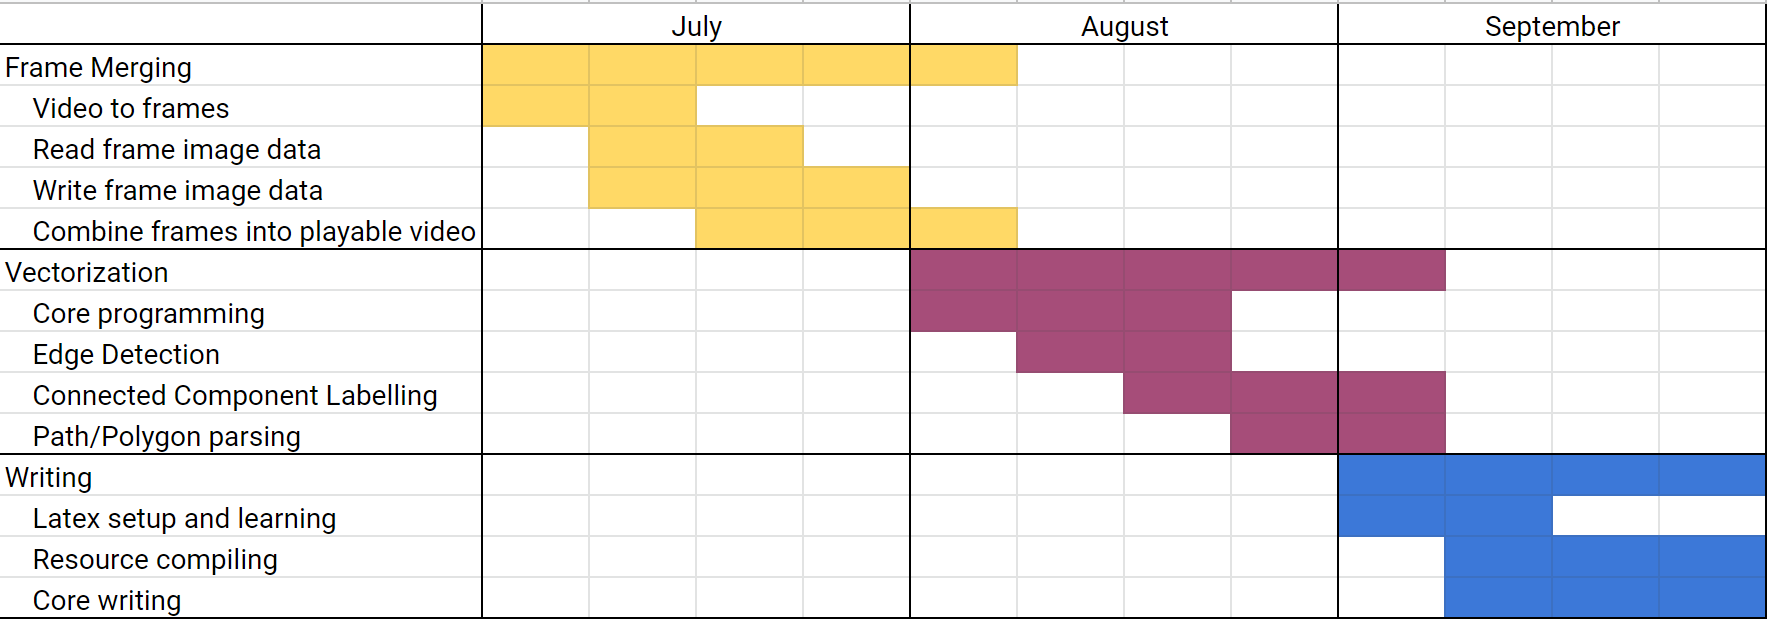
\includegraphics[scale=0.53]{Gantt.png}
        \end{center}
    \end{landscape}
    \pagebreak

    \pagebreak

    \subsection{Risks}\label{subsec:risks}

    \tab
    Naturally, a project of this scale that is very experimental in nature has many multi-faceted risks
    associated with it that can severely impact the development of the project if not correctly mitigated.
    \sentence
    As such, it is important to detect these risks as early as possible and have detailed and usable mitigation
    strategies to counter such risks and avoid their possibly devastating effects.
    \sentence
    Below are the risks listed and detailed with 4 key properties, first a detailed description to supplement the
    title of the risk.
    \sentence
    Then, a probability and consequentiality score out of 5 with 5 being the highest and 1 being the lowest.
    \sentence
    Finally, the mitigation strategy that would be used to offset and handle the consequences of the risk.

    \paragraph{Bad Time Management}
    \begin{itemize}
        \item Description: Time is not managed well or correctly and development falls behind schedule
        \item Probability: 5
        \item Consequentiality: 3
        \item Mitigation: Define a safe schedule with large buffer zones early on and skip and tasks taking too long
        to complete
    \end{itemize}

    \paragraph{Data Loss}
    \begin{itemize}
        \item Description: Data is lost as a result of some hardware failure and/or negligence
        \item Probability: 1
        \item Consequentiality: 5
        \item Mitigation: Back up all data using online services like GitHub as well as external drives
    \end{itemize}

    \paragraph{Tools Too Difficult}
    \begin{itemize}
        \item Description: Tools and libraries used are too difficult to use or learn
        \item Probability: 2
        \item Consequentiality: 4
        \item Mitigation: Ensure familiarity with tools beforehand by reading and experimenting before project
        development
    \end{itemize}

    \paragraph{Tools Not Helpful}
    \begin{itemize}
        \item Description: Tools and libraries are not being cooperative and are slowing down development
        \item Probability: 4
        \item Consequentiality: 2
        \item Mitigation: Ensure using popular tools with strong community, ensure familiarity with tools beforehand,
        use alternative tools if possible or necessary
    \end{itemize}

    \paragraph{Catastrophic fatal disaster}
    \begin{itemize}
        \item Description: By some horrible disaster an intergalactic alien invasion finally commences on earth and
        the aliens aim directly and only on my working space destroying all equipment and data
        \item Probability: 1
        \item Consequentiality: 5
        \item Mitigation: Ensure backups of all data are made on services like GitHub and on external drives and
        continue work on an external machine or using online tools
    \end{itemize}

    \paragraph{Personal issues}
    \begin{itemize}
        \item Description: Personal or family issues get in the way of development causing delays or prolonged
        periods of inefficiency
        \item Probability: 4
        \item Consequentiality: 4
        \item Mitigation: Ensure that some work is done at least every day in order to ensure no loss of momentum and
        keep in touch with supervisor to update with progress or any issues
    \end{itemize}

    \paragraph{Poor results}
    \begin{itemize}
        \item Description: Results are not promising or motivating and project proves to be more difficult than
        anticipated
        \item Probability: 3
        \item Consequentiality: 4
        \item Mitigation: Ensure that the most research and effort is made during the project and make clear the
        significant effort put as well as the difficulty of the project within the final document
    \end{itemize}

    \subsection{Testing}\label{subsec:testing}

    \tab
    Testing is an important part of software engineering, as it allows developers to ensure that the program behaves
    as expected even after changes to the code, this means that refactors or new implementations can easily be done
    since any breaking changes will fail the tests that previously passed.
    \sentence
    This makes developing new changes or code more reliable since there is a pillar of trust knowing that if the
    tests pass, then the software is behaving correctly, assuming of course the tests are well written and defined.
    \sentence
    In order to ensure that the application is behaving in the expected way, the project needed some kind of
    testing facilitation.
    \sentence
    A variety of classic testing methodologies and philosophies were used in this project namely, unit testing,
    integration testing and acceptance testing.

    \subsubsection{Unit Testing}\label{subsubsec:unit-testing}

    \tab
    The first testing methodology used was none other than the classic and simple unit testing.
    \sentence
    In our case we used a variety of classic automated unit tests, in-code \code{assert} statements and regular
    logging messages each serving different purposes.
    \sentence
    Firstly, the typical automated unit tests were used at the end of a computation to ensure that the output image
    was as expected, using whatever possible methods to do this.
    \sentence
    One of the ways was to test the output image's properties such as resolution, bit depth, size, distinct colors,
    among others.
    \sentence
    Secondly, in-code \code{assert} statements were used before any requirement that was needed to be true before
    computation, usually with regards to expected inputs.
    \sentence
    While this is not a traditional testing method, it was used as such here as there are many times where the input
    is not guaranteed to meet the requirements and thus a graceful failure is the only option with detailed messages.
    \sentence
    Finally, regular logging messages were used throughout the processing.
    \sentence
    These were used less as hard tests and more as indicators of less critical correct or incorrect behavior and very
    often used to measure time passed for every phase or step as execution times became fairly long.
    \sentence
    These three techniques were all used to ensure that the application was tested from the lowest point possible and
    the developer is able to understand how the code is being run and when and why it may be failing.

    \subsubsection{Integration Testing}\label{subsubsec:integration-testing}

    \tab
    Since many phases and process had to interact with one another and pass data to each other, it was important to
    ensure that this was behaving correctly using integration testing.
    \sentence
    In this case, a process such as average edge detection for example would have a specific output that perhaps the
    next process, edge based CCL, may not be expecting or may not know how to behave with.
    \sentence
    In addition to the core concepts were used from unit testing such as using in-code \code{assert} statements
    and logging statements, additional code was added in order to ensure that the application would either use the
    same data formats, or have a trustworthy converter to convert the data.
    \sentence
    An excellent is example is OpenCV's \code{Mat} type representing a matrix which was used during edge detection
    but the next steps would only know how to handle a built in type representing images.
    \sentence
    Thus, a converter was created to ensure that whenever the \code{Mat} type was used it was immediately converted
    to the internal type ensuring that the entire application would be uniform in what data types it would use and
    expect.
    \sentence
    Using integration testing using measures like these, we can ensure that the application can have components and
    processes interact with one another in the expected and correct behavior.

    \subsubsection{Acceptance Testing}\label{subsubsec:acceptance-testing}

    \tab
    Perhaps the most used and most important methodology used in this project was acceptance testing.
    \sentence
    In this case specifically this was done manually while developing in order to ensure results are visually as
    expected.
    \sentence
    This is because this is a graphics based project after all and the final judge as to whether the image is correct
    or not, is of course the human eye.
    \sentence
    A typical test case here was to run some computation on a frame, (have a coffee because it took a while) and
    check to see if the output image was something that was at least close to what was expected.
    \sentence
    This was how the majority of the main important validation was done since no automated test can ever tell if an
    image is acceptable.
    \sentence
    Indeed, there were many cases where the output image would have the expected properties such as resolution, color
    depth, size reduction etc and yet still be nothing more than noise because of some oversight or bug in the code.
    \sentence
    Thus, it is safe to say that while unit testing and integration testing were extremely important in this project,
    the true most important testing methodology used in this project was that which uses the the human eye and that
    being acceptance testing.

    \pagebreak


    \section{Evaluation}\label{sec:evaluation}

    \tab
    In order to know when the program is behaving correctly and to evaluate how well it is performing its task, we
    need to define some evaluation methods and metrics.
    \sentence
    Essentially there really only exist two key traits to the process, how accurate is the process and how well is
    the compression.
    \sentence
    A possible third angle could be performance, but this was never a priority to begin with and this can be heavily
    optimized and improved later, not to mention that it will differ across machines and architectures.
    \sentence
    Thus we will only discuss and detail the two key evaluation properties, accuracy and compression.

    \subsection{Accuracy}\label{subsec:accuracy}

    \tab
    The first property to evaluate is accuracy, or more accurately (pun intended), the lossy-ness that is incurred
    from the process.
    \sentence
    As mentioned earlier, since the vectorization process is transforming data from one form of representation to
    another, there will be data loss, especially if one intends to reduce size as we do.
    \sentence
    However, since we are aiming for \italic{Visually Lossless Compression}, it is important to know how to measure
    this data lossy-ness accurately in a meaningful way.
    \sentence
    Below we detail the two methods of evaluating the accuracy of an image using quantitative methods and qualitative
    methods.

    \subsubsection{Quantitative Methods}\label{subsubsec:quantitative-methods}

    \tab
    The quantitative methods we can use to evaluate the accuracy of the process are fairly straightforward since
    really all that we need to do is compare the data of both images, the input and the output.
    \sentence
    As such, we can relatively easily loop over every pixel in the original image and compare the color of that pixel
    to the color that is visible at that coordinate within the output SVG image.
    \sentence
    While vector graphics do not use the concept of pixels, we can still go to a specific coordinate on the image and
    query the color visible their using our own means.
    \sentence
    It is important to note here that 100\% may not only be impossible, but in fact is actually not ideal as we are
    not aiming for a truly lossless transformation.
    \sentence
    What we are aiming for is a \italic{Visually Lossless} transformation, meaning any data loss should be invisible
    to the human eye.
    \sentence
    Therefore, while quantitative methods for accuracy are quick and easy, they do not accurately represent the true
    goal of this project, which was never aimed to be lossless.

    \subsubsection{Qualitative Methods}\label{subsubsec:qualitative-methods}

    \tab
    The qualitative methods of comparing accuracy are the most meaningful and important but at the same time, the
    most difficult to measure and make sense of.
    \sentence
    Really, the main judge of whether a compression algorithm is \italic{Visually Lossless} is the human eye, but
    measuring perceived quality and difference has complications.
    \sentence
    However, despite being difficult to accurately measure, as after all, visual perception differs amongst people
    and "quality" can be subjective, there are ways to measure this and make \italic{some} informed conclusion based
    on the data.
    \sentence
    This of course can be done by using a sample set of different people with as diverse possible perception and
    notion of "quality" as possible.
    \sentence
    Despite being very difficult and expensive to gather such a sample set (especially in these times), a sample set
    of close friends and family of fairly diverse ages and backgrounds was gathered and used to measure perceived
    accuracy.

    \subsection{Compression}\label{subsec:compression}

    \tab
    The other property to evaluate is compression rate, i.e., the size ratio of the new file's size to the original
    file's size.
    \sentence
    It is important to note that the project's aim with regard to compression in that the aim is to have smaller file
    sizes \italic{and} scalability, that means there may be instances where file size may actually become larger,
    like when dealing with a low resolution input.
    \sentence
    However, that same output file can now be used on higher resolution displays with no issues, whereas the original
    cannot and any upscaled copies of the original will never be as small in size as our output, at least that is the
    aim.
    \sentence
    Thus, the upscaling factor needs to be taken into account when viewing the data in order to gain a fuller
    understanding of the whole picture.
    \sentence
    Below we detail the many different quantitative methods that can be used to evaluate the compression of the process.

    \subsubsection{Quantitative Methods}\label{subsubsec:quantitative-methods2}

    \tab
    Compression can really only be quantitatively measured but it can be measured fairly easy and therefore, we can
    gather a large amount of data to gain a more concrete understanding of the compression rate of the
    process especially when considering upscaling.
    \sentence
    The major thing to take note of the compression ratio or the cost savings, they are two numbers meaning the same
    thing, how much storage was saved after the compression process.
    \sentence
    But worth taking into account the fact that we are attempting to add upscaling to the equation, meaning upscaled
    versions of an image should be compared against our own to show a true measure of how much savings were made not
    just from the single original image but also against higher resolution images.
    \sentence
    This is because the vector graphics image will always be scalable wheras for higher resolution displays we
    require higher resolution images to properly view them, thus it is fair to compare the vector graphics image
    against a copy of the original image in a higher resolution.

    \pagebreak


    \section{Results}\label{sec:results}

    \tab
    Results have been relatively mixed and have been both extremely motivating and extremely disappointing such that
    much of the development process itself was very heavily affected by the results.
    \sentence
    Overall, the process shows that it is feasible to perform this very well with \italic{theoretical} high levels of
    accuracy with relatively small file sizes.
    \sentence
    However, there is always a key issue preventing the success from being fully met and ready to celebrate.
    \sentence
    Raster graphics are flawed in their nature, to divide an image into a grid of colors will always be lossy and
    inaccurate and add to that any effects that are added in post processing to help make the image clearer or less
    jagged, then there is even more data lost.
    \sentence
    The image becomes clear to the human eye from its resolution but so much data was lost and altered to achieve
    this, data that any process such as vectorization would have a very difficult time reconstructing.
    \sentence
    This was shown especially when using Color based CCL where over 95\% of all regions had less than 5 pixels in
    them because those were new pixels added for anti-aliasing, an effect added between edges to make them less
    jagged to the eye.
    \sentence
    Rasterization added data that was never there that the vectorization process now has to find and undo, this is
    why the project became much harder than anticipated, because of this deadly realization.

    \begin{figure}[h!]
        \centering
        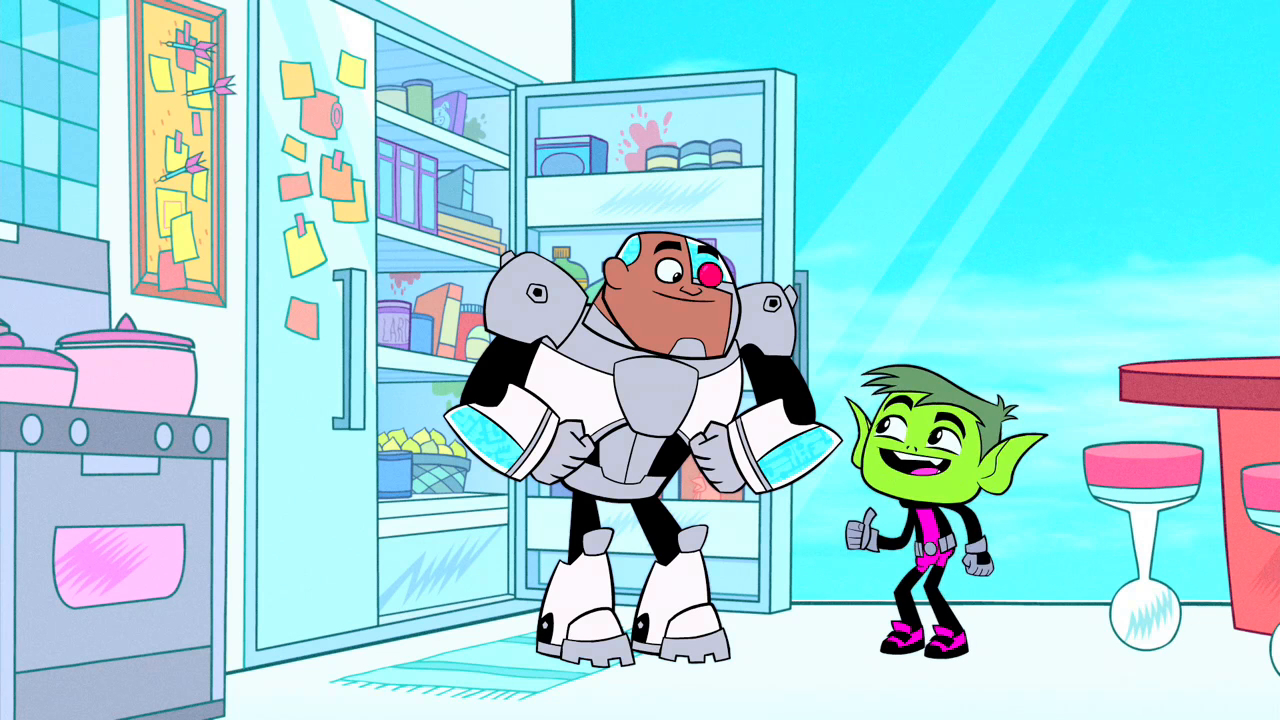
\includegraphics[width=\textwidth]{OriginalFrame.png}
        \caption[OriginalFrame]{Original image, a frame from \italic{Teen Titans Go!} 1MB}
        \label{fig:originalframe}
    \end{figure}

    \begin{figure}[h!]
        \centering
        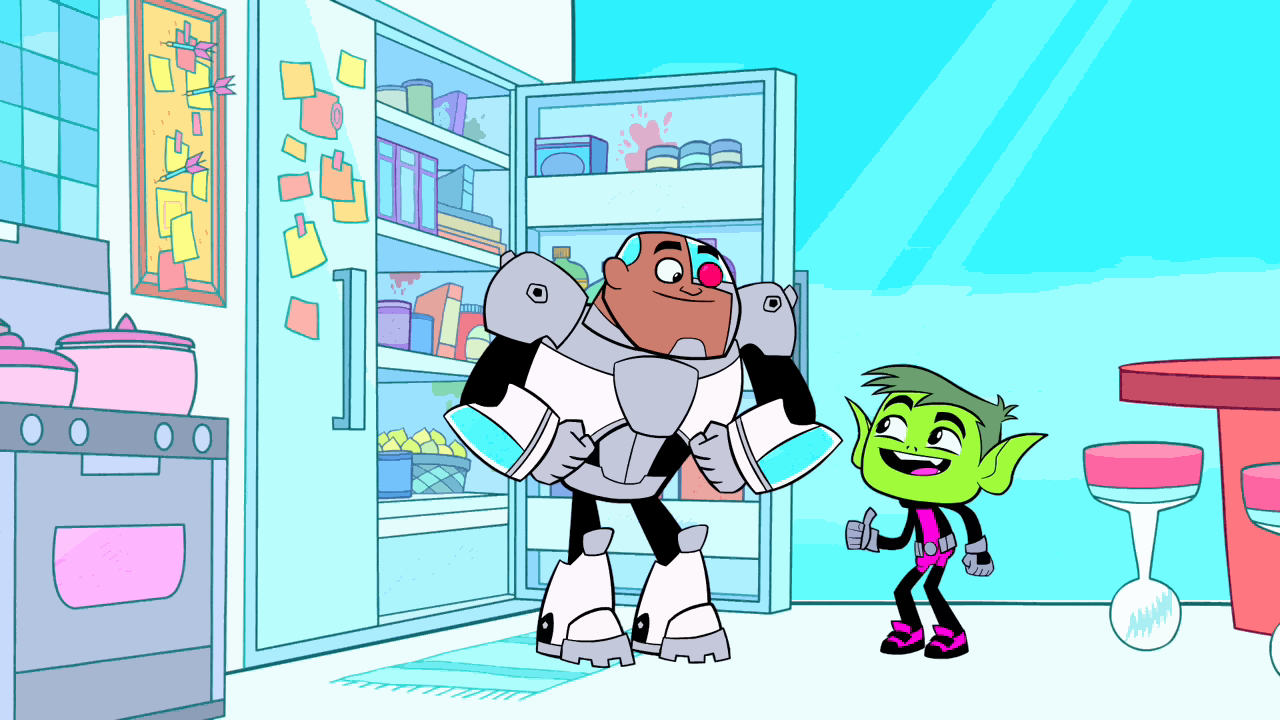
\includegraphics[width=\textwidth]{CCL.png}
        \caption[CCL]{Image after Color based CCL, an impressive 336kb meaning ~70\% savings but note some minor data
        loss in the clouds background, oven window and fridge drawer}
        \label{fig:CCL}
    \end{figure}

    \begin{figure}[h!]
        \centering
        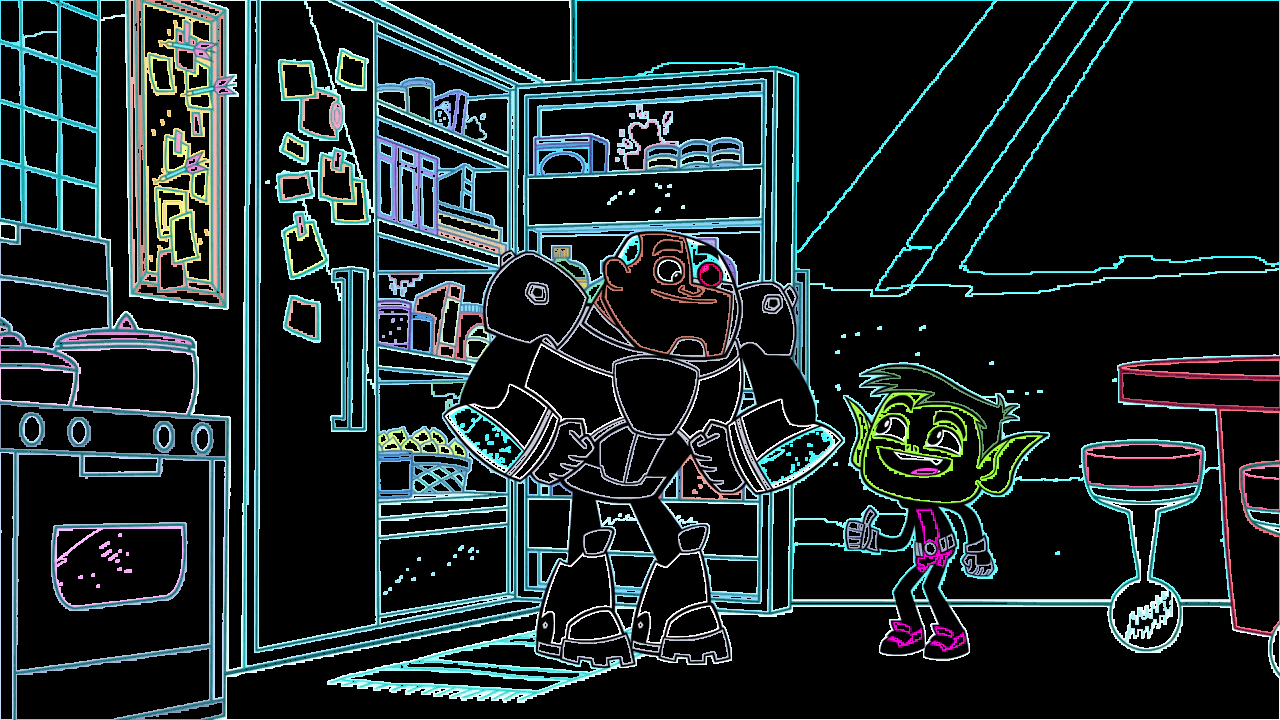
\includegraphics[width=\textwidth]{SmallComponents.png}
        \caption[SmallComponents]{Highlighting the components less than 5 pixels in size shows that edges of color
        regions seem to be the culprit of problems, these are the pixels in between colors, those that are added by
        anti-aliasing}
        \label{fig:smallcomponents}
    \end{figure}

    \pagebreak


    \section{Challenges}\label{sec:challenges}

    \tab
    As shown by the previous sections in this document, this project has been far from trivial, in fact it was much
    more difficult and challenging than initially anticipated despite already expecting a high level of difficulty.
    \sentence
    While the project has been overall a very mentally stimulating, rewarding and fulfilling project it is important
    to note some of the major challenges that were faced during the development.
    \sentence
    This serves the purpose to inform future readers and those interested in this project about some of the
    challenges faced and how to either overcome them early, or more likely, to expect and prepare for them.
    \sentence
    While some of these issues can be mitigated earlier with further planning and research, the most difficult and
    major challenges are those inherent to the vectorization process and conversion of raster graphics.

    \subsection{Toolchain}\label{subsec:toolchain2}

    \tab
    Arguably the most preventable and frustrating challenges faced were those that were a direct result of the
    toolchain used, especially when there exist other tools that do not have these problems.
    \sentence
    The most frustrating of these is the lack of maturity in the JavaScript ecosystem.
    \sentence
    This can be seen with the very minimal Node.js standard library which contains only the most necessary built in
    functionality and instead delegates anything else to libraries, frameworks and other open source contributors.
    \sentence
    While this does have benefits it also has major disadvantages especially coming from the vast ecosystems of the
    JVM and Android which both come with large fully featured but modular standard libraries that provide standard
    ways to perform common operations.
    \sentence
    This weakness is shown extensively whilst using any JavaScript collections such as Array, Set or Map, which
    provide only the most basic functionality leaving common operations like copying and adding an element to an
    index up to the user or to some external dependency.
    \sentence
    However, perhaps the best example for an argument of the JavaScript ecosystem's immaturity is the fact that
    JavaScript supports object oriented concepts, including classes and methods, but does not allow programmers to
    declare when two objects are equal or not.
    \sentence
    The Set collection contains only distinct elements by first checking if an element already exists before
    inserting it and ignores it if it already exists.
    \sentence
    JavaScript does not allow the programmer to determine how this equality is checked which is done using === by
    default, instead, if the programmer wants a Set of custom objects they have to implement this themselves or
    use an external library, further adding to dependency hell.
    \sentence

    \bigskip
    Another issue from the toolchain used that was also completely unexpected and mostly taken for granted coming
    from the JVM world is the lack of true concurrency or multithreading in Node.js and JavaScript in general.
    \sentence
    Node.js is asynchronous meaning execution can jump between functions and wait until functions are complete by
    using the \code{Promise} API in addition to the \code{async} / \code{await} model.
    \sentence
    However, JavaScript does not allow multiple threads of execution at once and the only way to achieve this is by
    using multiple JavaScript instances, in the case of Node.js multiple Node processes which adds a huge amount of
    complexity to the program.
    \sentence
    This meant that any possible optimizations that could be made would be much more difficult than expected and
    would take too long to develop.
    \sentence
    This is an issue because the application can make use of parallel execution and can heavily benefit from this but
    because of the issues with the toolchain, such benefits would be too costly to achieve.
    \sentence
    These are just some of the examples of when the toolchain used was actively discouraging and slowing down
    development and this is something that was a major challenge and annoyance during development as it was not
    expected and is out of our direct control.

    \subsection{Performance}\label{subsec:performance}

    \tab
    Another major challenge was the performance of the program and trying to improve it in some way.
    \sentence
    Because of the desired accuracy and compression and the complexity and number of operations that are required to
    achieve these two key traits, the cost was performance since the program was just too complex.
    \sentence
    This was mostly expected at first, however what was not expected was the difficulty in optimizing and reducing
    the time it took to run the process on a single frame and any added code would only compound the problem.
    \sentence
    This meant that in order to test some new code worked a full loop had to be run first before further proceeding,
    this would take anywhere between 5 to 10 minutes to finish and as a result productivity was much lower than
    desirable.
    \sentence
    How to improve this was obvious since there were two clearly possible solutions to take, add multithreading as
    only one thread was running and the CPU was maxing at only 9\% utilization, or use the GPU wherever possible as
    much of the code can theoretically be run on the GPU for insanely better results.

    \bigskip
    \sentence
    Adding multi-threading to the application was much more difficult than anticipated as the toolchain used simply
    did not allow for this to be an easy solution as mentioned in the above section~\fullref{subsec:toolchain2}.
    \sentence
    However, more beneficially perhaps was to use the GPU wherever possible as the GPU is capable of having huge
    performance improvements if the code is written for it.
    \sentence
    Indeed, the GPU was used in some parts of the application leading to truly shocking results, what took 60--100
    seconds now takes 4--6 seconds, however the difficulty and learning curve for correct and effective GPU
    programming is enormous.
    \sentence
    This really creates a very difficult decision to make because GPU optimizations are big cost big reward
    optimizations that can significantly increase productivity and in the long run provide us with more time to write
    and test code.
    \sentence
    In the end however, the time cost to rewrite code to run on the GPU was simply too high to risk and the
    potentially huge optimizations and performance improvements were not fully accomplished, thus, the program having
    very poor performance overall despite attempts to rectify this.

    \pagebreak


    \section{Reflection}\label{sec:reflection}

    \tab
    After working on this project over the last few months, it is important to look back and reflect on the
    experience to see what was learned and what new experiences were made.
    \sentence
    Firstly, the unexpected difficulty of the project and the continuous roadblocks and negative results have been
    extremely humbling and have been excellent experiences in development struggle and hardship;
    struggle is an excellent teacher and this project was a huge struggle.
    \sentence
    The main thing learned is patience and a new desire and appreciation for experimentation, even if the results
    will not go according to plan and the time and effort spent was high, the experience of the challenge is by far
    the greatest reward.
    \sentence
    Secondly, and more concretely, the technical knowledge that was gained through this project within both the
    computer graphics field and also in the JavaScript ecosystem in general are extremely valuable.
    \sentence
    Computer graphics is a complex and daunting field full of intense knowledge and technicality and had it not been
    for this project so much knowledge and experience within the field would have never been gained.

    \bigskip
    Having said all this however, it is important to mention what would be done differently if starting from the
    beginning, something that future readers interested in this kind of project should take important note of.
    \sentence
    Perhaps the most important thing to change is the toolchain from Node.js to one that allows true multithreading
    but with the same vast ecosystem as JavaScript.
    \sentence
    The first alternative that comes to mind is the JVM platform with its large thriving ecosystem, multiple languages
    to choose from (Java, Kotlin, Scala etc) and the addition of true multithreading, this is the ideal toolchain to
    use instead of a JavaScript based one.
    \sentence
    The other thing to note before starting over is to appreciate and comprehend the difficulty of this project and
    this problem.
    \sentence
    Vectorization is not an easy process and particularly so on complex media such as cartoons, even if they contain
    qualities that are favorable towards vectorization.
    \sentence
    In knowing this beforehand one may face less frustrations and have better expectations on what it means to achieve any
    decent results because while those results may not seem perfect, they are far more impressive than they seem.
    \sentence
    All in all however, the experience has been rewarding, fulfilling, mentally stimulating and a truly challenging
    adventure that is very much worth the time and effort to invest in simply for the experience and knowledge alone.

    \pagebreak


    \section{Future Work}\label{sec:future-work}

    \tab
    Despite being given many months to work on this project, it would be dishonest to claim that it is close to being
    completed, as there are still many future endeavours and tasks that can be completed given more time.
    \sentence
    These tasks were left out as they were either lower priority or out of the scope of the project's initial aims
    and objectives and were thus cut for time saving.
    \sentence

    \subsection{Optimization}\label{subsec:optimization}

    \tab
    As discussed in the preceding sections, one of the main issues with the project currently is the
    performance of the processing.
    \sentence
    This was never a high priority to begin with as it was clear early on that in order to aim for high accuracy and
    high compression, more instructions needed to be executed and thus more time was needed to execute them.
    \sentence
    However, given more time this is an angle that is important to investigate and tackle as the more complex the
    process becomes, the longer it takes to view any results, leading to significantly lower productivity.
    \sentence
    One of the main ways this can be achieved is by using the machine's hardware more efficiently especially by using
    more of the resources and making use of the many processing cores most modern machines possess today.
    \sentence
    As discussed earlier, the libraries and tools are not helpful in this regard thus either more work would be done
    in order to achieve this with the given tools, or a tool migration may be needed to fully leverage the power of
    other platforms such as the JVM when it comes to concurrency and multi-threading.

    \subsection{Future Research}\label{subsec:future-research}

    \tab
    Towards the end of the development cycle many new ideas began to make themselves apparent especially
    after the multiple consecutive failures to show major positive results.
    \sentence
    These ideas were noted and left aside in order to focus on the main goal of the project as they strayed slightly
    from the scope of the project and would have required more than the given time in order to truly explore correctly.
    \sentence
    However, given more time, these ideas should be further explored and tested as they can show further positive
    results and shed some light and insight onto the vectorization problem.
    \sentence
    The most important idea is the potential mixing of raster and vector graphics in a new graphics format in order
    to leverage the best of both formats and attempt to solve the issues of both.
    \sentence
    A potential algorithm would identify easily vectorizable areas of an image that would alter the data of the
    original image only less than a given maximum data loss threshold.
    \sentence
    These areas of the image would be vectorized and represented in vector graphics.
    \sentence
    Then, for the areas where vectorization fails to yield any positive results, usually because of noise,
    rasterization artifacts such as anti-aliasing or other non-vectorizable qualities such as gradients, the
    algorithm would keep those areas as raster pixel-based.
    \sentence
    As is made obvious by the simplistic high-level explanation, this idea is still not well thought out or
    researched, but given more time this is something that can be explored and researched in depth.

    \pagebreak


    \section{Conclusion}\label{sec:conclusion}

    \tab
    Finally, we conclude by summarizing what this document has gone over and provide some final thoughts and
    statements with regards to the impact that this project may have on the world, now and in the future.
    \sentence
    Vectorization is an already well established form of transforming graphics data from raster to vector with a lot
    of existing research and implementations that provide high quality results.
    \sentence
    However, all of them have some inherent flaws, with newer machine-learning based ones inheriting the flaws of
    machine learning with them, and older ones requiring human input for color, or just completely ignoring color
    entirely.
    \sentence
    This project aimed at remedying the problem by experimenting with possible solutions to this problem tackling it
    from an angle specifically based on animated cartoons to have a well established expected input and output.
    \sentence
    Results were mixed in that they showed the possibility and feasibility of such a solution especially one that
    uses no machine learning and requires minimal input.
    \sentence
    But results were always lacking in some form leaving much to be desired and introducing more questions and
    problems than answers and solutions.
    \sentence
    However, despite these results, it is absolutely possible that given more time to develop and optimize and
    research more into this problem, more potential avenues for this problem will be found to be used as a basis to
    finally solve this problem.
    \sentence
    With that solution, we can hope that timeless animated cartoons like \italic{Tom and Jerry} and \italic{The
    Fairly OddParents} which have brought happiness and meaning to millions of lives across generations and borders
    will continue to do so for many more generations to come.

    \pagebreak

    \bibliographystyle{ieeetr}
    \bibliography{bib}

    \pagebreak

\end{document}